
\documentclass[12pt]{article} % Use A4 paper with a 12pt font size - different paper sizes will require manual recalculation of page margins and border positions

% Generated with LaTeXDraw 2.0.8
% Mon Jun 17 19:00:40 EDT 2013
\usepackage[usenames,dvipsnames]{pstricks}
\usepackage{epsfig}
\usepackage{pst-grad} % For gradients
\usepackage{pst-plot} % For axes
\usepackage[left=1.3cm,right=4.6cm,top=1.8cm,bottom=4.0cm,marginparwidth=3.4cm]{geometry} % Adjust page margins
\usepackage{amsmath} % Required for equation customization
\usepackage{amssymb} % Required to include mathematical symbols
\usepackage{xcolor} % Required to specify colors by name
\usepackage{amsthm}
\usepackage{float}
\usepackage{tikz}
\usetikzlibrary{shapes,backgrounds,trees}
\usepackage{wasysym}

\makeatletter
\newcommand{\mytag}[2]{%
  \text{#1}%
  \@bsphack
  \protected@write\@auxout{}%
         {\string\newlabel{#2}{{#1}{\thepage}}}%
  \@esphack
}
\makeatother

\setlength{\parindent}{0cm} % Remove paragraph indentation
\newcommand{\tab}{\hspace*{2em}} % Defines a new command for some horizontal space
%\newcommand{\choose}[2]{\left(\begin{matrix}
%{#1}\\{#2}
%\end{matrix}\right)}
\date{}
\title{Introduction to Probability Theory - Lecture 10}
%----------------------------------------------------------------------------------------

\newtheorem{defn}{Definition}
\newtheorem{example}{Example}
\newtheorem{prop}{Proposition}
\newtheorem{exer}{Exercises}
\newtheorem{thm}{Therorem}
\begin{document}
\maketitle
\section{Variance}
In our last lecture, we defined expectation and noted some of its important properties. Today, we define variance and do the same.
\begin{defn}
Let $X$  be a random variable. We define the \emph{variance} of $X$ to be
$$Var(X) = E\left(\left(X - E(X)\right)^2\right)$$
\end{defn}
In other words, the variance is the expected value of the squared deviations from the mean. A useful theorem is:
\begin{thm}
$$Var(X) = E(X^2)-\left(E(X)\right)^2$$
\end{thm}
\begin{proof}
\begin{eqnarray*}
Var(X) &=& E\left(\left(X - E(X)\right)^2\right)\\
&=& E\left(X^2 - 2XE(X)+\left(E(X)\right)^2\right)\\
&=& E(X^2) - E(2XE(X))+E(\left(E(X)\right)^2)\\
&=& E(X^2) - 2\left(E(X)\right)^2+\left(E(X)\right)^2\\
&=& E(X^2) - \left(E(X)\right)^2
\end{eqnarray*}
\end{proof}
The following are some important properties of the variance:
\begin{itemize}
\item $$Var(X+c) =Var(X) \textrm{ for } c \textrm{ a constant}.$$
\item $$Vacr(cX) = c^2 Var(X) \textrm{ for } c \textrm{ a constant}.$$
\item If $X$ and $Y$ are independent, then
$$Var(X+Y) = Var(X) + Var(Y)$$
\item $Var(X)$ is NOT linear!
\item $Var(X)\geq0$ with equality only if $X$ is a constant (not random). 
\end{itemize}
We will continue to use expectation and variance in our study of random variables and their distributions. For this reason, there are no assigned problems in chapter 4. We will now move on to examine continuous random variables.
\section{Continuous Random Variables}
There are several ways to define what it means for a random variable to be continuous. The text uses the following:
\begin{defn}
A random variable is continuous (or has a continuous distribution) if its CDF is differentiable.
\end{defn}
Or, we may say:
\begin{defn}
A random variable is called continuous if there exists $f(x)$ such that the CDF is given by:
$$F(X) = \int_{-\infty}^x f(t) dt$$
\end{defn}
Either way, we define the \emph{probability density function} or pdf in the following manner:
\begin{defn}
For a continuous random variable with CDF $F(x)$, the probability density function is given by:
$$\frac{d}{dx}F(X) = f(x)$$
\end{defn}
This is consistent with the Fundamental Theorem of Calculus, which describes the relationship between definite integrals and derivatives.\\\\
Intuitively speaking, we want to think of a continuous random variable as one whose \emph{support} is not discrete. (Recall that the support of a random variable are the values at which it has non-zero probability). We think of discrete as meaning 'gaps between numbers', like the integers: 1,2,3, etc. = there are many numbers between them. It is also true that there are many numbers between two rational numbers, so that a random variable whose possible values are all rational numbers is still discrete. For a random variable to be continuous, we need it to have non-zero probability on some interval on the real line.\\\\
This fundamental difference between continuous and discrete random variables leads to a somewhat different specification of probability. In particular, the pdf $f(x)$ does NOT specify a probability at $X=x$. Rather, it specifies a \emph{density} of probability at $X=x$, and integrating over an interval yields the probability that $X$ takes a value in that interval. More precisely:
\begin{defn}
If $X$ is a continuous random variable with pdf $f(x)$, 
$$P(a<X<b) = \int_a^b f(x) dx$$
\end{defn}
As can be inferred from the above definition:\\\\

\emph{The probability that a continuous random variable takes any single value is ZERO!}\\\\
Also, the endpoints $a$ and $b$ 'don't matter', in that:
$$P(a\leq X\leq b) = P(a<X\leq b)= P(a<X<b)= P(a\leq a<b)$$

Recall from calculus that the definite integral of a(n integrable) function $f$ over an interval $[a,b]$ is the area under the curve of the graph of $f$. Thus, if $X$ is a continuous random variable with pdf $f(x)$, we can visualize the probability that $X$ takes a value in the interval $[a,b]$ as shown:\\

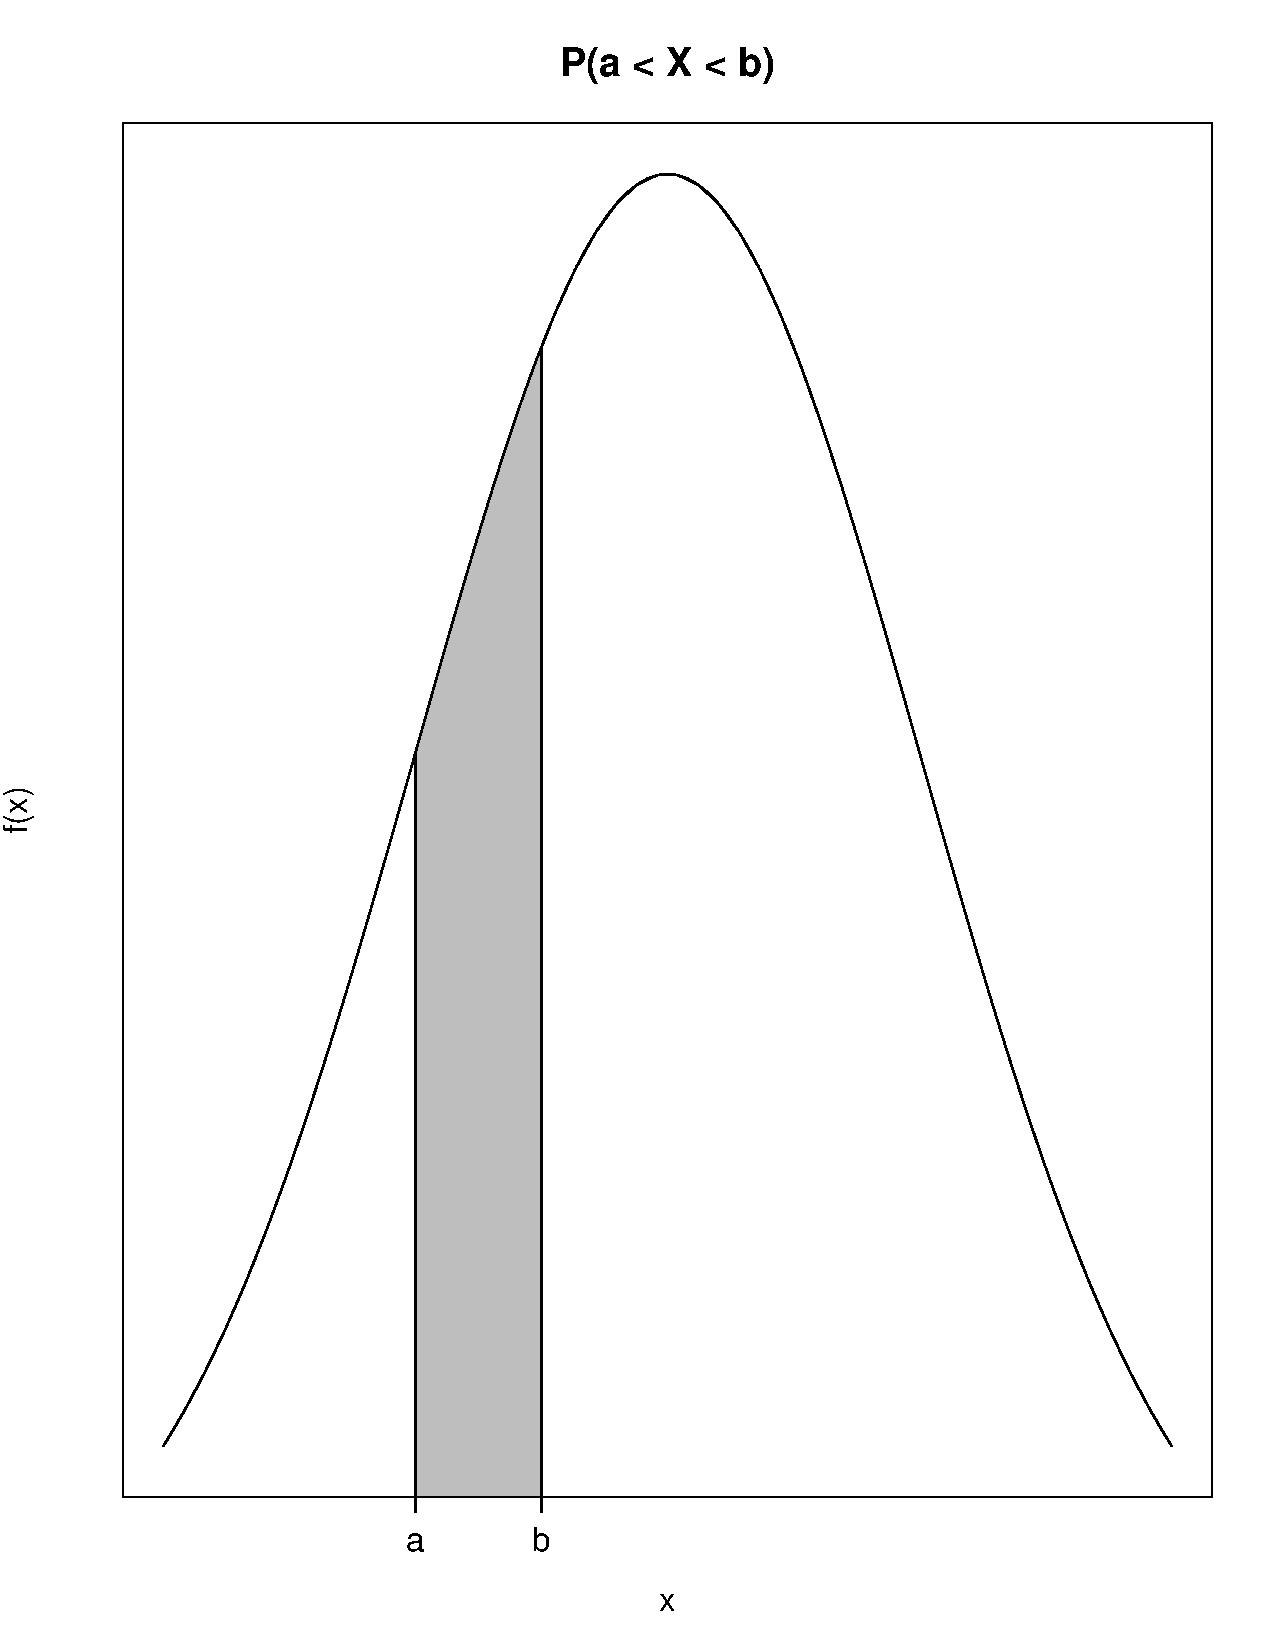
\includegraphics[height=3in]{area.pdf}

Now, there are some requirements that a valid probability density must satisfy:\\
\begin{thm}
A valid pdf must satisfy:
\begin{enumerate}
\item $$f(x) \geq 0$$
\item $$\int_{-\infty}^\infty f(x) dx = 1$$
\end{enumerate}
\end{thm}
\begin{proof}
\begin{enumerate}
\item If $f(x_0)<0$, then $f(x)<0$ in a neighborhood (interval) around $x_0$, leading to a negative probability.\\
NOTE: This is the proof as the book states it. This is only true if we assume $f(x)$ is \emph{continuous} at all $x$. Technically, $f$ can be negative at a point $x_0$, so long as that is a point of discontinuity. In other words, $f$ can be negative on a  \emph{discrete} set, because those are points with zero probability.  We won't belabor this point, but it is important (to me!) to be technically correct.
\item $$\int_{-\infty}^{\infty} f(x) dx = P(-\infty<X<\infty) = 1$$
\end{enumerate}
\end{proof}
Note that any $f$ that satisfies the above is a valid pdf for some random variable.\\\\
The book has a few examples of continuous distributions that are not among the ones we will focus on (logistic and Rayleigh). 
\section{Expectation for Continuous Random Variables}
\begin{defn}
Let $X$ be a continuous random variable with pdf $f(x)$. The expectation of $X$ is defined to be:
$$E(X) = \int_{-\infty}^{\infty} x f(x) dx$$
\end{defn}
This is analogous to the discrete case, with the sum replaced by an integral. The continuous version of expectation satisfies the same properties as expectation in the discrete case. Namely:
\begin{itemize}
\item $E(X)$ is a measure of center
\item $E(X)$ is linear
\item For a function $g:\mathbb{R}\rightarrow \mathbb{R}$, 
$$E(g(X)) = \int_{-\infty}^{\infty} g(x) f(x) dx$$
\end{itemize} 

We will now examine some common continuous distributions, derive some of their major properties and point out some special facts about each.

\end{document}